\documentclass[a4paper]{article}
\usepackage{listings}
\usepackage{inconsolata}
\usepackage{courier}
\usepackage{setspace}
\usepackage{hyperref}
\usepackage{Sweave}
\begin{document}
\Sconcordance{concordance:capm_example.tex:capm_example.Rnw:%
1 6 1 1 0 38 1 1 2 4 0 1 2 2 1 1 2 4 0 1 2 2 1 1 2 8 0 1 1 12 0 1 2 1 1 %
1 2 1 0 1 1 12 0 1 2 1 1 1 2 4 0 1 2 1 1 1 2 12 0 1 2 1 1 1 2 5 0 1 3 1 %
1 1 2 1 0 1 1 7 0 1 1 12 0 1 2 2 1 1 2 13 0 1 2 1 1 1 2 1 0 2 1 8 0 1 2 %
1 1 1 2 1 0 1 1 17 0 1 1 3 0 1 2 2 1 1 2 4 0 4 2 4 0 3 2 4 1 1 2 10 0 1 %
2 1 1 1 2 9 0 1 2 1 1 1 3 5 0 1 2 1 1 1 2 21 0 1 2 1 1 1 2 24 0 1 2 1 1 %
1 2 1 0 4 1 3 0 1 2 1 1 1 4 3 0 2 1 3 0 1 2 1 1 1 2 7 0 1 2 1 0 1 1 14 %
0 1 1 18 0 1 1 12 0 1 2 9 1 1 7 9 0 1 2 2 1 1 8 10 0 1 2 5 1 1 4 6 0 1 %
2 1 1 1 2 4 0 4 2 4 0 3 2 4 1 1 2 24 0 1 2 3 1 1 4 3 0 1 1 18 0 1 1 3 0 %
3 2 1 4 3 0 1 1 18 0 1 1 3 0 3 2 3 1 1 4 3 0 1 1 3 0 3 2 1 4 3 0 1 1 3 %
0 3 2 7 1 1 2 1 0 1 1 25 0 1 1 22 0 1 1 3 0 1 2 1 1 1 2 4 0 2 2 5 0 2 2 %
4 0 2 2 5 0 1 2 3 1 1 8 10 0 1 2 4 1 1 2 1 0 1 1 25 0 1 1 22 0 1 1 3 0 %
1 2 1 1 1 4 1 2 5 0 1 2 1 4 1 2 5 0 1 2 3 1 1 8 10 0 1 2 9 1}

\setlength{\parskip}{.5cm}
\title{An introduction to \texttt{capm}: an R package for companion animal population management}
\author{Oswaldo Santos, Fernando Marques,\\ Marcos Amaku and Fernando Ferreira}
\date{May 24, 2013}
\maketitle 
\begin{center}
oswaldosant@gmail.com
\end{center}

Human-companion animal interaction is a non free of problems ubiquitous phenomenon. To avoid adverse consequences in public health and animal welfare contexts, it is essential to have companion animal population management programs, focused on responsible ownership. Although there had been multiple initiatives around the world to control animal populations, the effect of those initiatives is unknown in most of the cases and the problem is still present. Academic claims regarding the lack of data can be found in literature since 1990s and nowadays, the need of objective assessments is a consensus. 

The \texttt{capm} package is an initiative to guide and automate quantitative analysis relevant for companion animal population management. For the first version of \texttt{capm} (0.01-1), functions can be broadly categorized in two groups:\\
\begin{itemize}
\item Survey design and demographic characterization.
\item Intervention-oreinted models in population dynamics.
\end{itemize}

The \texttt{capm} package is intended for specific analysis under a predefined workflow. Those interested in the implementation of new models or survey designs may want to consult available options in other packages (see for example: \texttt{deSolve, FME, rootSolve, GillespieSSA and survey}).

The objective of this mansucript is to present a worked example which ilustrate the workflow that can be facilitated by \texttt{capm} package. Deitailed options of functions are not discussed but the reader can consult their help pages. The example combine real spatial data from Santos district (Brazil) and hypotetical dog demographic data. Why hypoyhetical data? Previous (Amaku et al., 2009; 2010; Ferreira 2010) and ongoing (Santos, 2013) studies of our research group did not take in to account variables that now we deem that must be assessed to better understand and guide population management programs. Therfore, we simulated data hopefully will serve as a guide for future studies. 

We are aware of the limitations imposed by lack of different resources to support population management programs, a fact that often result in incomplete datasets. This situation is  addresed in the example and consequences of completeing datasets with "guess" estimates are quantified.

The \texttt{capm} package version 0.01-1 is an instance of the evolution of companion animal population management and this means that it is a process (infinitely) far to be finished. The feedback to improve available functions and suggest new ones certanly will produce great advances in the package evolution.

The developement version is available on \url{https://github.com/oswaldosantos}. Additional documentation such as tutorials and even a shiny ("point and click") interface will also be available in this site.

\section{Population study of owned dogs in urban area of Santos district}

In this worked example, a pilot study will be designed to estimate the total number of dogs per household and with this variable, the sample size and composition of a complex sample design will be estimated. Using sample data, demographic characteristics of owned dogs will be estimated and then, population dynamics will be modeled to assess the effect of current dog population management strategies. Global and local sensitivity analysis will be made to quantify the importance of all variables, including those which where not considered in the sample design. In this way, prarameters can be ranked to guide the definition of intervention priorities. Finally, intervention scenarios will be simulated to assess the effect of differente strategies.

\subsection{Pilot study}
To begin, define the composition of a two-stage cluster sampling design of arbitrary (expereince-based) size, selecting 20 primary sampling units (psu) with probability proportional to size and with replacement (ppsr). Within each psu, select 5 secondary sampling units (ssu) through systematic sampling. psu and ssu correspond to census tracks (setores censit\'{a}rios in portuguese) and households (domic\'{i}lios in portuguese) respectively.

In the web page of the Instituto Brasileiro de Geografia e Estat\'{i}stica \url{www.ibge.gov.br} it is possible to download the shapefiles and spreadsheets of the 2010 national census. Subsets of the needed data are included in the \texttt{capm} datasets and will be used for the sake of simplicty.

The first step is to load the \texttt{capm} package.
\begin{Schunk}
\begin{Sinput}
> library(capm)
\end{Sinput}
\end{Schunk}


Load the \texttt{psu.ssu} file which contain a list of all psu and their sizes.
\begin{Schunk}
\begin{Sinput}
> data(psu.ssu)
\end{Sinput}
\end{Schunk}

The id of each psu is in the first column and the number of ssu (its size) in the second one.

\begin{Schunk}
\begin{Sinput}
> str(psu.ssu)
\end{Sinput}
\begin{Soutput}
'data.frame':	649 obs. of  2 variables:
 $ psu: num  3.55e+14 3.55e+14 3.55e+14 3.55e+14 3.55e+14 ...
 $ ssu: int  119 43 79 129 53 46 176 281 409 317 ...
\end{Soutput}
\begin{Sinput}
> print(head(psu.ssu), digits = 15)
\end{Sinput}
\begin{Soutput}
              psu ssu
1 354850005000001 119
2 354850005000002  43
3 354850005000003  79
4 354850005000004 129
5 354850005000007  53
6 354850005000008  46
\end{Soutput}
\end{Schunk}

Select 20 psu with ppsr. If you want a *.csv file with the results, set \texttt{write} equal to \texttt{TRUE}.
\begin{Schunk}
\begin{Sinput}
> selected.psu = ppssr(psu.ssu, 20)
> head(selected.psu)
\end{Sinput}
\begin{Soutput}
     selected.psu size
1 354850005000170  206
2 354850005000011  281
3 354850005000656  220
4 354850005000103  272
5 354850005000456  253
6 354850005000476  214
\end{Soutput}
\end{Schunk}

In each of the selected psu, select 5 ssu through systematic sampling. Again, you can get a *.csv file with the results.
\begin{Schunk}
\begin{Sinput}
> selected.ssu = siss(selected.psu, 5)
\end{Sinput}
\end{Schunk}

Let's see the first 3 psu. Note that you have the specific ssu that must be surveyed.
\begin{Schunk}
\begin{Sinput}
> selected.ssu[, 1:3]
\end{Sinput}
\begin{Soutput}
     354850005000170 354850005000011 354850005000656
[1,]               6              16              41
[2,]              47              72              85
[3,]              88             128             129
[4,]             129             184             173
[5,]             170             240             217
\end{Soutput}
\end{Schunk}

Create *.kml files to see on GoogleEarths those psu that must be surveyed. Keep in mind that the \texttt{mplyer} object is just the name of the file and in case it is in a directory other than the current working directory, the path to the file muste be specified. In this case, we specify a \texttt{capm} file.
\begin{Schunk}
\begin{Sinput}
> mplyer <- system.file('shp/santos.shp', package="capm")
> #psukml(mplyer, selected.psu[, 1], 1)
\end{Sinput}
\end{Schunk}

Supose that you made the pilot and are ready to work on the final survey. Fisrt, take a look of the collected data. Remember that each row represent a household.
\begin{Schunk}
\begin{Sinput}
> data(pilot)
> str(pilot)
\end{Sinput}
\begin{Soutput}
'data.frame':	100 obs. of  2 variables:
 $ psu : Factor w/ 17 levels "354850005000080",..: 16 16 16 16 16 3 3 3 3 3 ...
 $ dogs: num  2 1 2 1 2 1 0 0 0 0 ...
\end{Soutput}
\begin{Sinput}
> head(pilot)
\end{Sinput}
\begin{Soutput}
              psu dogs
1 354850005000619    2
2 354850005000619    1
3 354850005000619    2
4 354850005000619    1
5 354850005000619    2
6 354850005000095    1
\end{Soutput}
\end{Schunk}

\subsection{Final survey}
Calculate the sample size and composition for the final survey using the defaults for \texttt{clus2}.
\begin{Schunk}
\begin{Sinput}
> clus2(psu.ssu, pilot, level = 0.95, error = 0.1, cost = 12)
\end{Sinput}
\begin{Soutput}
                                               Value
Sample size                             1.296000e+03
Number of psu to be sampled             3.240000e+02
Number of ssu to be sampled in each psu 4.000000e+00
Intercluster variance                   4.888107e+04
Intracluster variance                   8.030345e-01
Intraclass correlation coefficient      5.506181e-01
\end{Soutput}
\end{Schunk}

Select psu and ssu acording to previous results and create *.kml files. To avoid name conflicts with *.kml files of the pilot, move this files to other folder or delete them before creating the new files.
\begin{Schunk}
\begin{Sinput}
> f.selected.psu = ppssr(psu.ssu, 20)
> f.selected.ssu = siss(f.selected.psu, 5)
> psukml(mplyer, f.selected.psu[, 1], 1)
\end{Sinput}
\begin{Soutput}
 The maps are in the directory: 

 /home/oswaldo/Documents/Projects/capms/exemplo
\end{Soutput}
\end{Schunk}

Review the survey data before proceding.
\begin{Schunk}
\begin{Sinput}
> data(Sample)
> str(Sample)
\end{Sinput}
\begin{Soutput}
'data.frame':	1606 obs. of  12 variables:
 $ interview_id: int  1 2 3 3 4 5 6 6 7 7 ...
 $ psu         : num  3.55e+14 3.55e+14 3.55e+14 3.55e+14 3.55e+14 ...
 $ dogs        : num  1 0 1 1 0 0 1 1 1 1 ...
 $ sex         : Factor w/ 2 levels "Female","Male": 2 NA 1 1 NA NA 1 1 2 1 ...
 $ age         : int  5 NA 2 0 NA NA 4 12 0 12 ...
 $ castrated   : Factor w/ 2 levels "no","yes": 1 NA 1 2 NA NA 2 2 2 1 ...
 $ castrated1  : Factor w/ 2 levels "no","yes": 1 NA 1 2 NA NA 1 1 1 1 ...
 $ adopted     : Factor w/ 2 levels "no","yes": 1 NA 1 1 NA NA 2 1 1 2 ...
 $ births      : num  0 NA 0 2 NA NA 0 0 0 0 ...
 $ present     : Factor w/ 2 levels "no","yes": 2 NA 2 2 NA NA 1 2 1 2 ...
 $ death       : Factor w/ 2 levels "no","yes": 1 NA 1 1 NA NA 1 1 2 1 ...
 $ lost        : Factor w/ 2 levels "no","yes": 1 NA 1 1 NA NA 2 1 1 1 ...
\end{Soutput}
\begin{Sinput}
> ?Sample
\end{Sinput}
\end{Schunk}

\subsection{Population pyramids}
You can build population pyramids conditioned on age and sex or even on age, sex and reproductive status (castration). Just specify the \texttt{Sample} columns which contain this variables.
\begin{Schunk}
\begin{Sinput}
> pyramid(Sample, col.age = 5, col.sex = 4)
\end{Sinput}
\end{Schunk}
\begin{center}
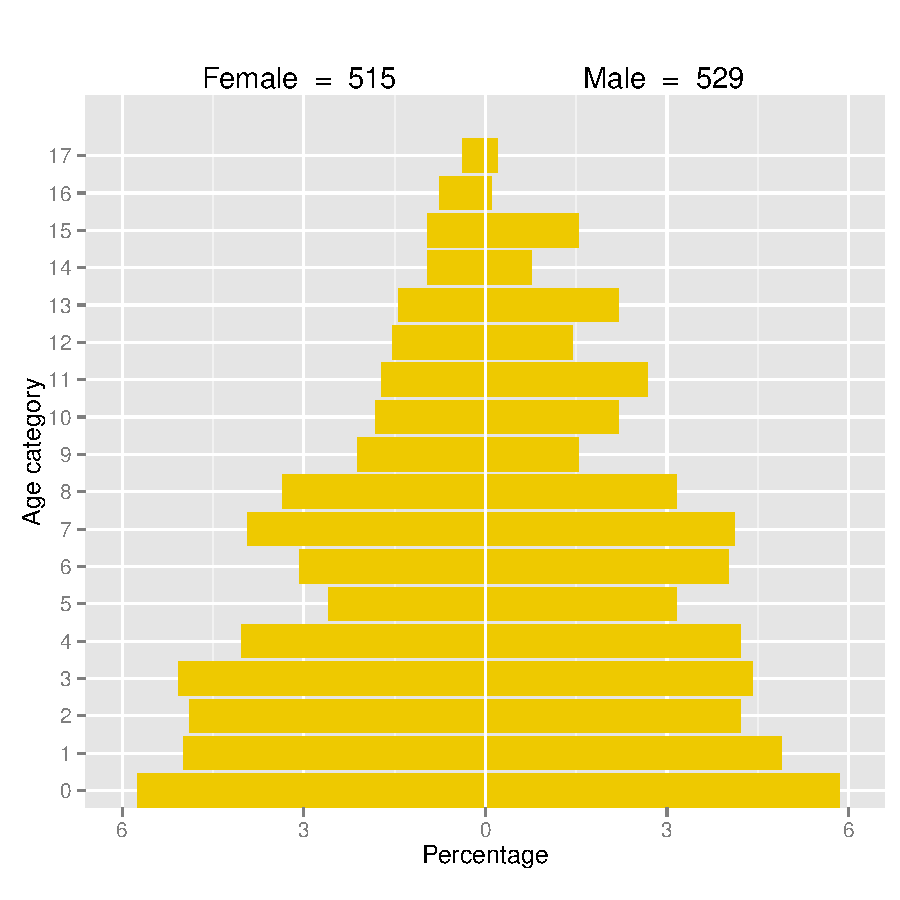
\includegraphics{capm_example-pyramids1}
\end{center}
\begin{Schunk}
\begin{Sinput}
> pyramid(Sample, col.age = 5, col.sex = 4, col.cas = 6)
\end{Sinput}
\end{Schunk}
\begin{center}
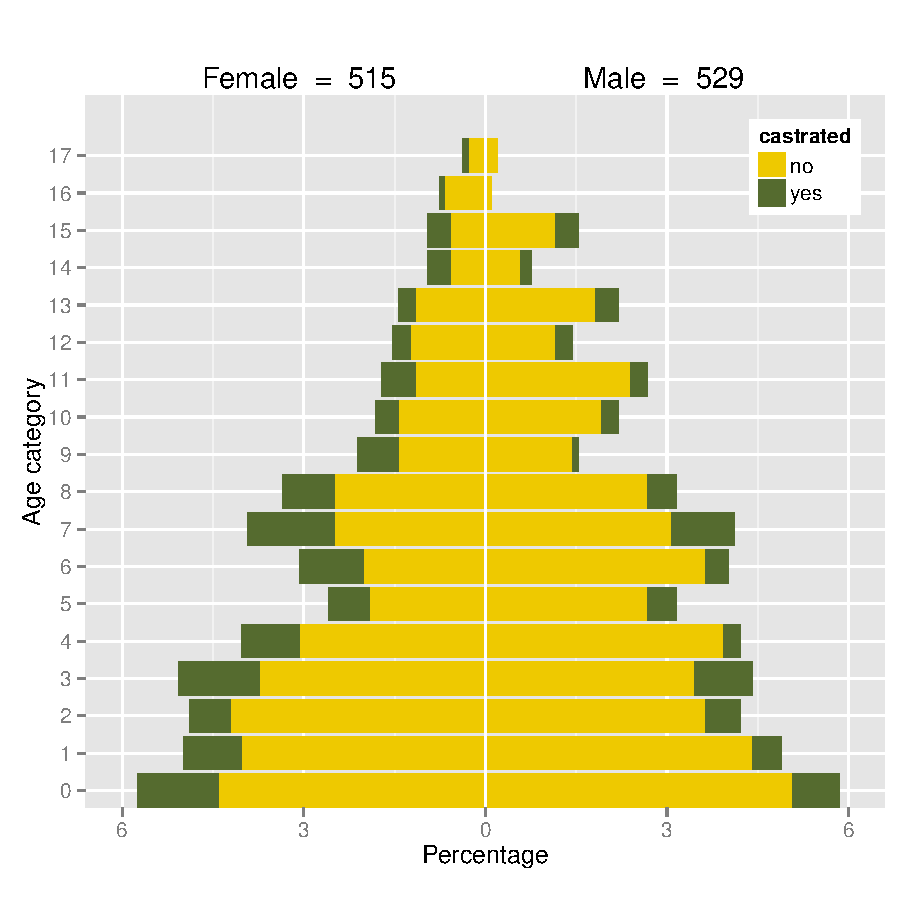
\includegraphics{capm_example-pyramids2}
\end{center}
\subsection{Estimates}
Now you are in position to estimate demographic parameters.

Specify the two-stage cluster design. For this, indicate the columns of \texttt{psu.ssu} containing the psu and ssu.
\begin{Schunk}
\begin{Sinput}
> (design = svyd2(psu.ssu, Sample, psu.col = 2, ssu.col = 1))
\end{Sinput}
\begin{Soutput}
2 - level Cluster Sampling design
With (231, 1296) clusters.
svydesign(ids = ~psu.id + ssu.id, weights = weights, fpc = ~pop.size + 
    psu.size, data = sample, ...)
\end{Soutput}
\end{Schunk}

Look at the variables contained in the survey design.
\begin{Schunk}
\begin{Sinput}
> names(design$variables)
\end{Sinput}
\begin{Soutput}
 [1] "psu.id"     "ssu.id"     "dogs"       "sex"        "age"       
 [6] "castrated"  "castrated1" "adopted"    "births"     "present"   
[11] "death"      "lost"       "pop.size"   "psu.size"  
\end{Soutput}
\end{Schunk}

Specify the type of estimate for each variable. As shown by the previous command, the first two and the last two variables are not to be estimated. Thus, use empty quotes to ingore it.
\begin{Schunk}
\begin{Sinput}
> variables = c("", "", "total", "prop", "mean", rep("prop", 3), 
+               "total", rep("prop", 3), "", "")
\end{Sinput}
\end{Schunk}

Make sure you specify the correct type of estimate for each variable.
\begin{Schunk}
\begin{Sinput}
> cbind(names(design$variables), variables)
\end{Sinput}
\begin{Soutput}
                   variables
 [1,] "psu.id"     ""       
 [2,] "ssu.id"     ""       
 [3,] "dogs"       "total"  
 [4,] "sex"        "prop"   
 [5,] "age"        "mean"   
 [6,] "castrated"  "prop"   
 [7,] "castrated1" "prop"   
 [8,] "adopted"    "prop"   
 [9,] "births"     "total"  
[10,] "present"    "prop"   
[11,] "death"      "prop"   
[12,] "lost"       "prop"   
[13,] "pop.size"   ""       
[14,] "psu.size"   ""       
\end{Soutput}
\end{Schunk}

Calculate the summary statistics for the survey.
\begin{Schunk}
\begin{Sinput}
> (estimates = svysumm(design, variables = variables, rnd = 3))
\end{Sinput}
\begin{Soutput}
                     Estimate       SE     2.5 %    97.5 %  Deff Error (%)
Total.dogs          89136.810 2303.976 84621.100 93652.520 1.746     5.066
Prop.sex.Female         0.497    0.016     0.465     0.529 1.132     6.461
Prop.sex.Male           0.503    0.016     0.471     0.535 1.132     6.380
Mean.age                5.684    0.148     5.393     5.975 1.209     5.117
Prop.castrated.no       0.802    0.013     0.775     0.828 1.192     3.276
Prop.castrated.yes      0.198    0.013     0.172     0.225 1.192    13.246
Prop.castrated1.no      0.952    0.007     0.937     0.966 1.195     1.487
Prop.castrated1.yes     0.048    0.007     0.034     0.063 1.195    29.254
Prop.adopted.no         0.904    0.010     0.885     0.923 1.150     2.111
Prop.adopted.yes        0.096    0.010     0.077     0.115 1.150    19.835
Total.births        21870.897 3243.138 15514.464 28227.330 1.230    29.064
Prop.present.no         0.155    0.012     0.132     0.179 1.178    15.272
Prop.present.yes        0.845    0.012     0.821     0.868 1.178     2.807
Prop.death.no           0.899    0.010     0.879     0.919 1.212     2.225
Prop.death.yes          0.101    0.010     0.081     0.121 1.212    19.828
Prop.lost.no            0.946    0.008     0.930     0.961 1.233     1.607
Prop.lost.yes           0.054    0.008     0.039     0.070 1.233    27.932
\end{Soutput}
\end{Schunk}

Estimates for subsets are also possible. For total estimates of \texttt{factor} variables, first transform it to \texttt{numeric}.
\begin{Schunk}
\begin{Sinput}
> sample1 = Sample[, c(1:4, 6:7, 11)]
> sample1[, 5] = as.character(sample1[, 5])
> sample1[which(sample1$castrated == "yes"), 5] = 1
> sample1[which(sample1[, 5] == "no"), 5] = 0
> sample1[, 5] = as.numeric(sample1[, 5])
\end{Sinput}
\end{Schunk}

Define the survey design in the usual way and then subset as required.
\begin{Schunk}
\begin{Sinput}
> design.sex = svyd2(psu.ssu, sample1,
+                    psu.col = 2,
+                    ssu.col = 1)
> design.f = subset(design.sex, sex == 'Female')
> design.m = subset(design.sex, sex == 'Male')
\end{Sinput}
\end{Schunk}

From here, procede as with previous estimates.
\begin{Schunk}
\begin{Sinput}
> names(design.sex$variables)
\end{Sinput}
\begin{Soutput}
[1] "psu.id"     "ssu.id"     "dogs"       "sex"        "castrated" 
[6] "castrated1" "death"      "pop.size"   "psu.size"  
\end{Soutput}
\begin{Sinput}
> variables.sex = c("", "", "total", "", "total",
+                   "prop", "prop", "", "")
> cbind(names(design.sex$variables), variables.sex)
\end{Sinput}
\begin{Soutput}
                   variables.sex
 [1,] "psu.id"     ""           
 [2,] "ssu.id"     ""           
 [3,] "dogs"       "total"      
 [4,] "sex"        ""           
 [5,] "castrated"  "total"      
 [6,] "castrated1" "prop"       
 [7,] "death"      "prop"       
 [8,] "pop.size"   ""           
 [9,] "psu.size"   ""           
\end{Soutput}
\begin{Sinput}
> (estimates.f = svysumm(design.f, variables.sex, rnd = 3))
\end{Sinput}
\begin{Soutput}
                     Estimate       SE     2.5 %    97.5 %         Deff
Total.dogs          44290.092 1914.929 40536.901 48043.284 7.887044e+31
Total.castrated     10864.901 1030.490  8845.177 12884.625 1.521000e+00
Prop.castrated1.no      0.931    0.012     0.907     0.955 1.237000e+00
Prop.castrated1.yes     0.069    0.012     0.045     0.093 1.237000e+00
Prop.death.no           0.896    0.015     0.867     0.925 1.210000e+00
Prop.death.yes          0.104    0.015     0.075     0.133 1.210000e+00
                    Error (%)
Total.dogs              8.474
Total.castrated        18.590
Prop.castrated1.no      2.599
Prop.castrated1.yes    35.179
Prop.death.no           3.218
Prop.death.yes         27.771
\end{Soutput}
\begin{Sinput}
> (estimates.m = svysumm(design.m, variables.sex, rnd = 3))
\end{Sinput}
\begin{Soutput}
                     Estimate       SE     2.5 %    97.5 %  Deff Error (%)
Total.dogs          44846.718 1801.999 41314.864 48378.571   Inf     7.876
Total.castrated      6807.759  854.627  5132.720  8482.798 1.507    24.605
Prop.castrated1.no      0.972    0.007     0.958     0.986 1.009     1.452
Prop.castrated1.yes     0.028    0.007     0.014     0.042 1.009    49.982
Prop.death.no           0.902    0.014     0.874     0.930 1.208     3.070
Prop.death.yes          0.098    0.014     0.070     0.126 1.208    28.275
\end{Soutput}
\end{Schunk}

\subsection{Population dynamics based on point estimates}
To model population dynamics, you will consider both, owned and stray populations.

You do not have information for the stray population and even for the owned one, you do not have all the information requiered to build the model. This is a common situation but does not mean you have to finish your analysis here (unless you want). You can replace the lacking statistical estiamtes, by "guesses" or expert estimates. In any case, the consequences of this will can (and must) be assessed.

First, define the state variables and parameters required by the model (you may want to see the help page of \texttt{iasa} function). 

The next is a posibility:

\begin{Schunk}
\begin{Sinput}
> state.iasa = c(
+    f1 = 33425.19, cf1 = 10864.901,
+    m1 = 38038.96, cm1 = 6807.759,
+    f2 = 3342.519, cf2 = 108.64901,
+    m2 = 3803.896, cm2 = 68.07759
+ )
\end{Sinput}
\end{Schunk}

The number of owned intect females and males and the proportion that were castrated (\texttt{f1, m1}) were obtained from \texttt{estimates} object previously created. For stray intact and castrated animals, sizes were defined as 10 \% and 1 \% of the owned animals respectively. This is a conservative estimate, taking into consideration studies that have estimated this proportion as 5 \% from field data. For strays, the proportion of castrated individuals was arbitrary set as 5 \%.

\begin{Schunk}
\begin{Sinput}
> pars.iasa = c(
+    b1 = 21870.897, b2 = 4374.179,
+    df1 = 0.104, dm1 = 0.098, df2 = 0.1248, dm2 = 0.1176,
+    sf1 = 0.069, sf2 = 0.05, sm1 = 0.028, sm2 = 0.05,
+    k1 = 98050.49, k2 = 8055.456, h1 = 1, h2 = .5,
+    ab = 0.054, ad = 0.1, v = 0.1
+ )
\end{Sinput}
\end{Schunk}

Regarding owned population parameters, the number of births and abandonment and replacement rates (\texttt{b1, ab, v}) were obtained from \texttt{estimates} object. Death and sterilization rates for females and males (\texttt{df1, sf1, dm1, sm1}) were obtained from \texttt{estimates.f} and texttt{estimates.m} objects. Mean harem size (\texttt{h1}) was set acording to literature (Ferreira, 2010). Carrying capacity ((\texttt{k1}) was defined as 10 \% greater than the current population size. For the stray population, the number of births ((\texttt{b2}) was set as 15 \% of the corresponding value in owned population and death rates ((\texttt{df2, dm2}) was set as 15 \% greater than corresponding parameters in owned population. Carrying capacity ((\texttt{k2}) was 10 \% greater than the current population size and mean harem size ((\texttt{h2}) reflected a polyandrous mating system. Adoption rates was arbitray set as 10 \%. The proportion of adopted dogs estimated in \texttt{estimates} was not used because this also include those dogs that make internal fluxes within owned population.



Now, run the model for 30 years
\begin{Schunk}
\begin{Sinput}
> iasa.pt <- iasa(pars = pars.iasa,
+                 state = state.iasa,
+                 time = 0:30)
\end{Sinput}
\end{Schunk}

and plot the results for owned and stray populations.
\begin{Schunk}
\begin{Sinput}
> plotmodel(iasa.pt, variable = "N1")
\end{Sinput}
\end{Schunk}
\begin{center}
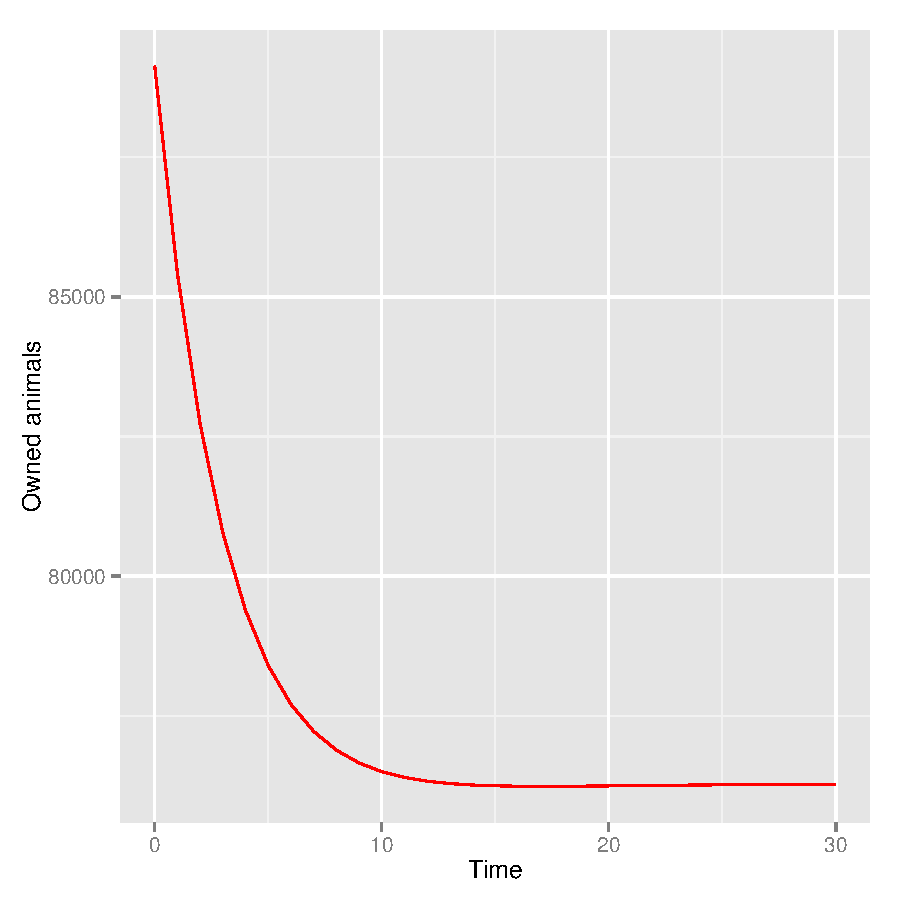
\includegraphics{capm_example-028}
\end{center}
\begin{Schunk}
\begin{Sinput}
> plotmodel(iasa.pt, variable = "N2")
\end{Sinput}
\end{Schunk}
\begin{center}
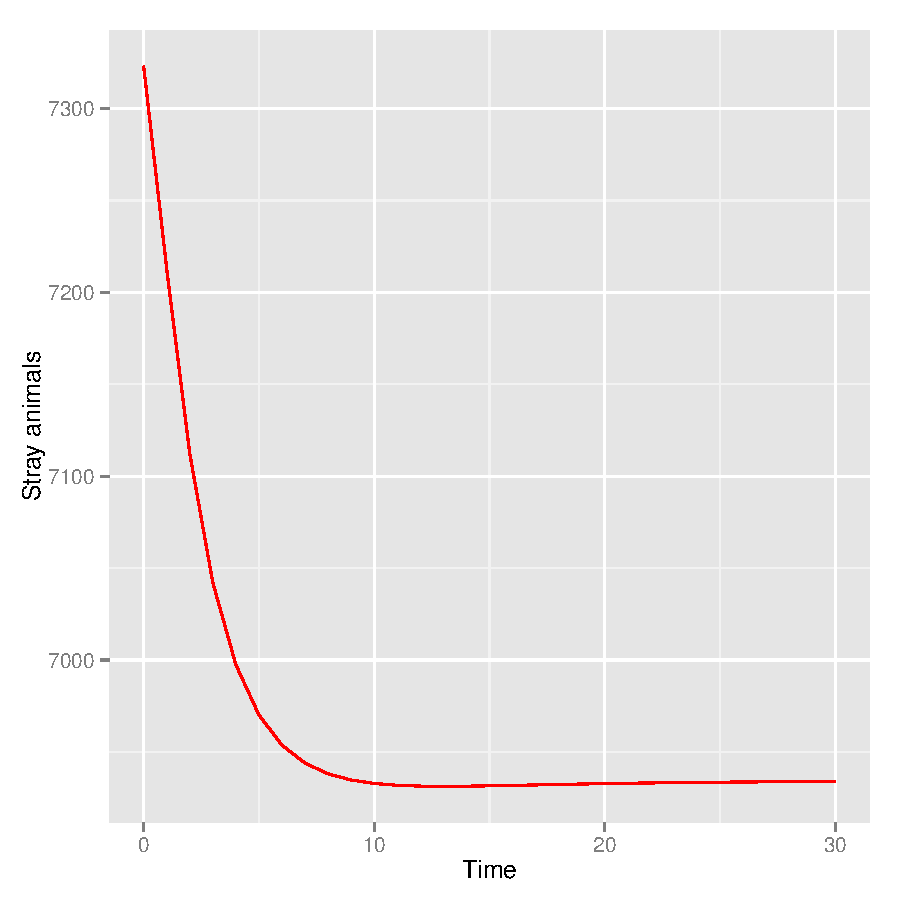
\includegraphics{capm_example-030}
\end{center}
\subsection{Global sensitivity analysis}
Previous figures represent the combination of parameters offered as a possibility. But what are the consequences of using the wrong values? To answer this question, make a global sensitivity analysis, varying the values in a range 10 \% (for example) greater and lesser than the point estimates.

Define the ranges.
\begin{Schunk}
\begin{Sinput}
> (par.rg.iasa10 = setranges(pars.iasa))
\end{Sinput}
\begin{Soutput}
            min          max
b1  19683.80730  24057.98670
b2   3936.76110   4811.59690
df1     0.09360      0.11440
dm1     0.08820      0.10780
df2     0.11232      0.13728
dm2     0.10584      0.12936
sf1     0.06210      0.07590
sf2     0.04500      0.05500
sm1     0.02520      0.03080
sm2     0.04500      0.05500
k1  88245.44100 107855.53900
k2   7249.91040   8861.00160
h1      0.90000      1.10000
h2      0.45000      0.55000
ab      0.04860      0.05940
ad      0.09000      0.11000
v       0.09000      0.11000
\end{Soutput}
\end{Schunk}

Because some parameters are small quantities, thier ranges are also small. An alternative is to use the estimated confidence intervals to build the ranges (see the \texttt{setranges} help page). \texttt{setranges} returns a \texttt{data.frame} and this means that you can define the ranges as you want.

Calculate and plot the global sensitivities for each parameter and for the combination of all parameters. First, analyse owned population sensitivities.
\begin{Schunk}
\begin{Sinput}
> glob.iasa.n1 = globalsens(
+   model.out = iasa.pt,
+   ranges = par.rg.iasa10, sensv = 'n1')
> head(glob.iasa.n1)
\end{Sinput}
\begin{Soutput}
    x     Mean       Sd      Min      Max      q05      q25      q50      q75
n10 0 71464.15   0.0000 71464.15 71464.15 71464.15 71464.15 71464.15 71464.15
n11 1 67284.74 119.6183 67079.31 67487.51 67100.11 67182.88 67285.43 67386.97
n12 2 64352.29 234.3142 63947.71 64747.33 63989.08 64153.07 64354.74 64552.81
n13 3 62326.66 334.5304 61746.42 62888.10 61806.26 62042.62 62331.49 62613.26
n14 4 60950.84 416.9409 60224.86 61647.86 60300.27 60597.26 60958.30 61308.37
n15 5 60034.61 481.7250 59193.02 60837.23 59280.99 59626.53 60044.65 60448.02
         q95 param
n10 71464.15    b1
n11 67467.48    b1
n12 64708.71    b1
n13 62833.67    b1
n14 61580.79    b1
n15 60760.49    b1
\end{Soutput}
\begin{Sinput}
> plotglobal(glob.iasa.n1)
\end{Sinput}
\end{Schunk}
\begin{center}
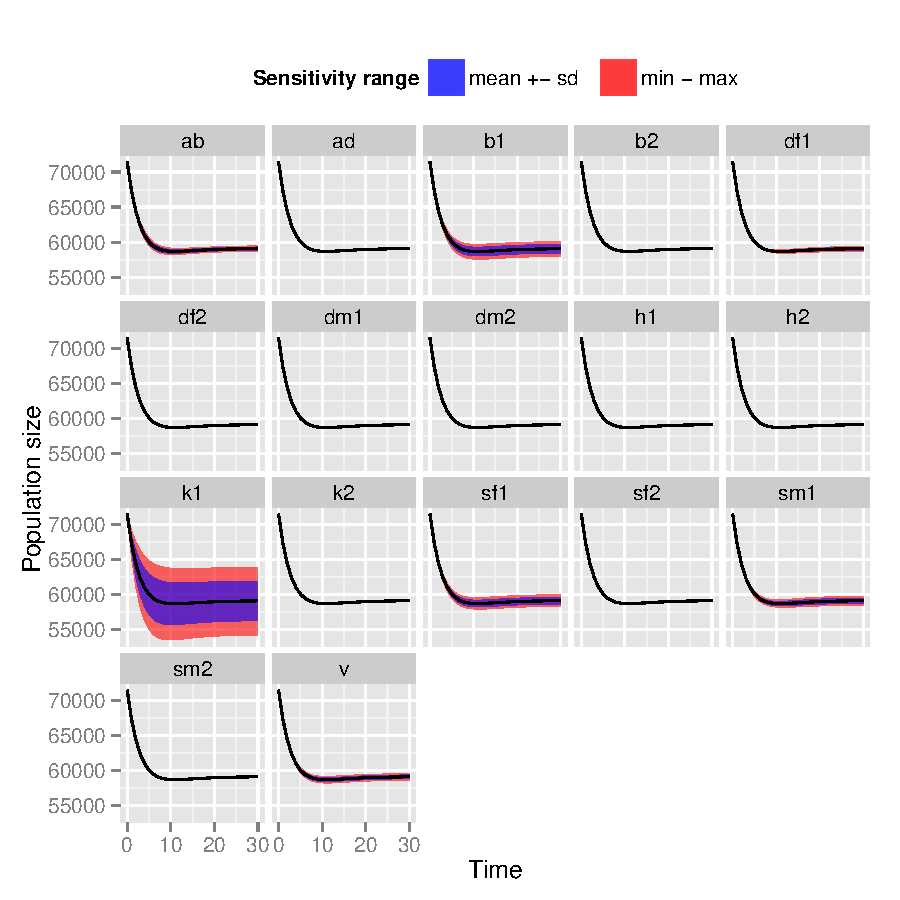
\includegraphics{capm_example-033}
\end{center}
\begin{Schunk}
\begin{Sinput}
> glob.iasa.all.n1 = globalsens(
+   model.out = iasa.pt,
+   ranges = par.rg.iasa10, sensv = 'n1', all = TRUE)
> head(glob.iasa.all.n1)
\end{Sinput}
\begin{Soutput}
    x     Mean       Sd      Min      Max      q05      q25      q50      q75
n10 0 71464.15    0.000 71464.15 71464.15 71464.15 71464.15 71464.15 71464.15
n11 1 67249.51 1212.260 65279.55 69830.81 65423.41 66170.46 67159.35 68228.45
n12 2 64300.69 2016.023 61078.97 68635.08 61355.66 62499.31 64098.47 65947.89
n13 3 62270.88 2533.315 58252.48 67765.88 58657.26 59903.67 61946.35 64359.52
n14 4 60897.63 2855.110 56402.76 67138.72 56827.96 58258.36 60479.65 63259.93
n15 5 59986.99 3046.612 55225.25 66689.93 55717.57 57275.37 59456.01 62510.07
         q95
n10 71464.15
n11 69183.61
n12 67499.63
n13 66266.75
n14 65372.76
n15 64731.64
\end{Soutput}
\begin{Sinput}
> plotglobal(glob.iasa.all.n1)
\end{Sinput}
\end{Schunk}
\begin{center}
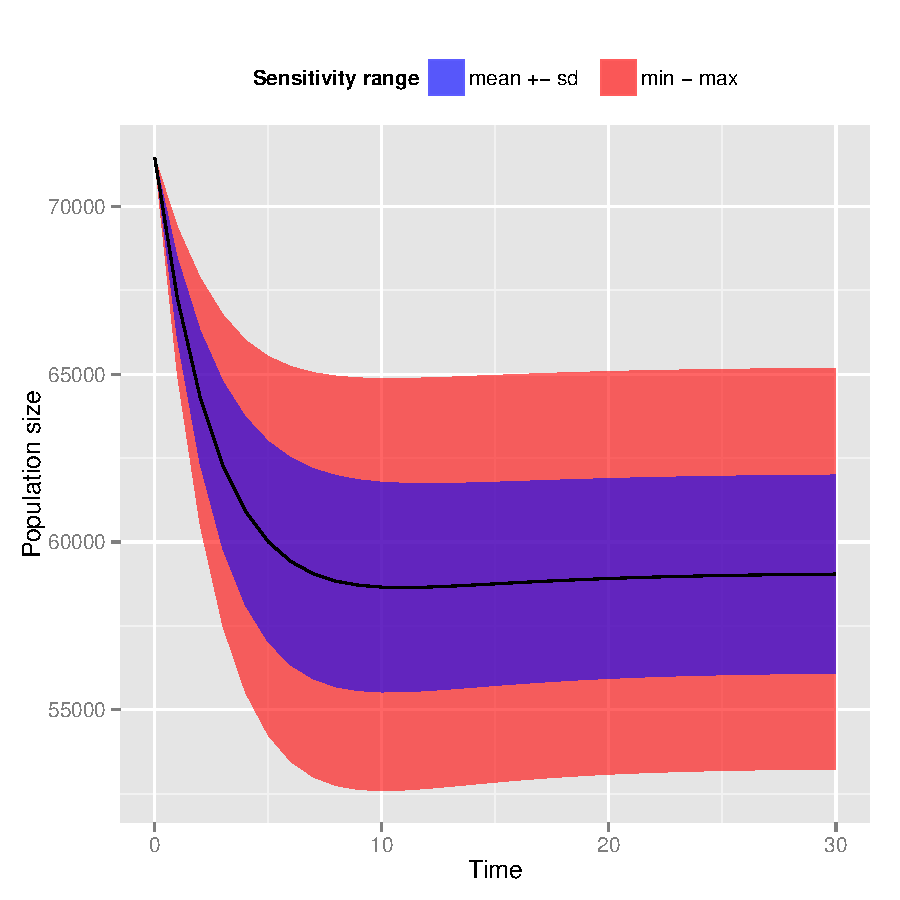
\includegraphics{capm_example-035}
\end{center}
As you can see, carrying capacity is by far the most influential parameter. Other influential parameters are abandonment rate, number of births and death, replacement and sterilizations rates. It must be noted that those parameters that were "guessed" have minimal influences on results.

Now, analyse stray population global sensitivities.
\begin{Schunk}
\begin{Sinput}
> glob.iasa.n2 = globalsens(
+   model.out = iasa.pt,
+   ranges = par.rg.iasa10, sensv = 'n2')
> plotglobal(glob.iasa.n2)
\end{Sinput}
\end{Schunk}
\begin{center}
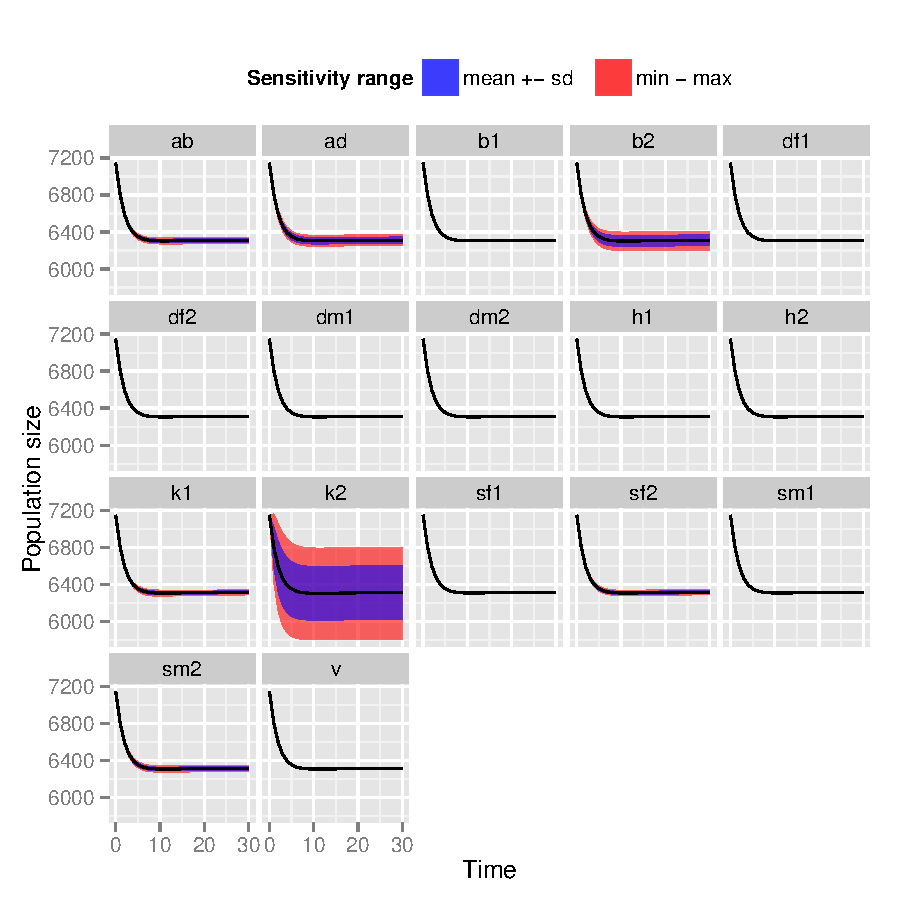
\includegraphics{capm_example-037}
\end{center}
\begin{Schunk}
\begin{Sinput}
> glob.iasa.all.n2 = globalsens(
+   model.out = iasa.pt,
+   ranges = par.rg.iasa10, sensv = 'n2', all = TRUE)
> plotglobal(glob.iasa.all.n2)
\end{Sinput}
\end{Schunk}
\begin{center}
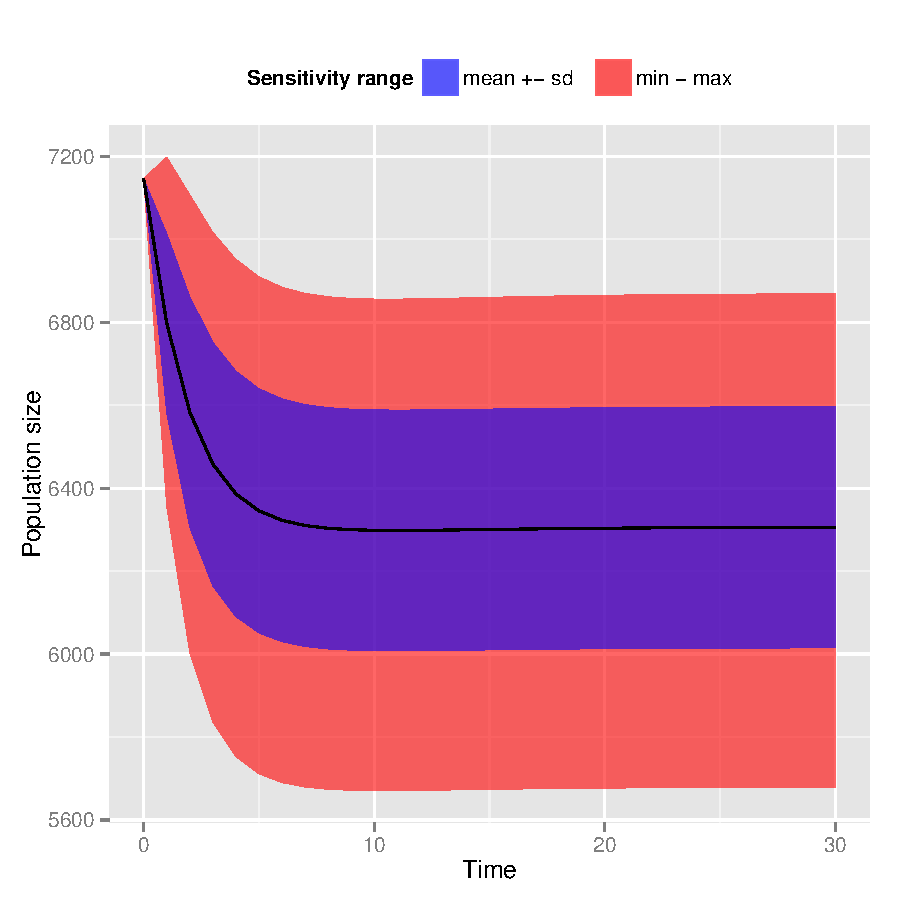
\includegraphics{capm_example-039}
\end{center}
Again, carrying capacity is the most influential parameter. A marked difference between both populations is that for the stray one, carrying capacity of the other population is influential as well as adoption rate. The number of births is of little importance and other parameters have no influence in practice.

Previous sensitivities can be interpreted in two ways. First, the more sensitive a parameter, the greater the need of precise estimates of it. Second, the more sensitive a parameter, the greater the priority in the context of population management programs.

\subsection{Local sensitivity analysis}
As a complement for global sensitivity analysis, local sensitivities allow the ranking of parameters according to their importance. Instead of using ranges, local sensitivities assess the parameters in a small space around the point estimates using the so-called sensitivity functions.

\begin{Schunk}
\begin{Sinput}
> local.iasa.n1 = localsens(model.out = iasa.pt, sensv = 'n1')
> head(local.iasa.n1)
\end{Sinput}
\begin{Soutput}
  x var       b1        b2        df1       dm1        df2        dm2       sf1
1 0  n1    0.000  0.000000    0.00000    0.0000  0.0000000  0.0000000     0.000
2 1  n1 2040.839  1.872831 -181.28403 -269.5802 -0.1514610 -0.1658255 -2061.918
3 2  n1 3997.167  6.835035 -137.35323 -415.6125 -0.4570163 -0.5182688 -3680.940
4 3  n1 5705.742 14.415855   62.17854 -467.8557 -0.7971679 -0.9491754 -4930.671
5 4  n1 7109.891 23.543544  355.29119 -456.4838 -1.0938244 -1.3909489 -5882.114
6 5  n1 8212.862 33.104152  693.65214 -406.6913 -1.3062148 -1.8111599 -6598.003
          sf2        sm1         sm2       k1       k2 h1 h2        ab
1   0.0000000     0.0000   0.0000000     0.00   0.0000  0  0     0.000
2  -0.8073403  -989.6155  -0.9396172 19690.42  24.9609  0  0 -3003.184
3  -3.1437594 -1834.3569  -3.7315476 32733.82  69.0452  0  0 -4686.747
4  -6.2525942 -2548.4717  -7.6358629 41079.47 111.6328  0  0 -5515.042
5  -9.4473580 -3149.1387 -11.9197648 46204.43 145.1335  0  0 -5815.341
6 -12.3217251 -3653.5405 -16.1207208 49180.87 168.5941  0  0 -5808.832
         ad         v
1   0.00000    0.0000
2  61.83909  914.9387
3 114.45023 1791.9893
4 156.30270 2557.9689
5 188.08736 3187.4697
6 211.23895 3681.9478
\end{Soutput}
\begin{Sinput}
> summary(local.iasa.n1)
\end{Sinput}
\begin{Soutput}
      value   scale      L1      L2     Mean     Min     Max  N
b1  2.2e+04 2.2e+04 9.3e+03 1.7e+03  9.3e+03     0.0 1.1e+04 31
b2  4.4e+03 4.4e+03 6.5e+01 1.3e+01  6.5e+01     0.0 8.5e+01 31
df1 1.0e-01 1.0e-01 2.4e+03 4.7e+02  2.3e+03  -181.3 3.4e+03 31
dm1 9.8e-02 9.8e-02 1.5e+02 3.5e+01 -4.7e+01  -467.9 1.1e+02 31
df2 1.2e-01 1.2e-01 1.5e+00 3.4e-01  7.8e-01    -1.4 3.6e+00 31
dm2 1.2e-01 1.2e-01 4.5e+00 9.1e-01 -4.5e+00    -7.6 0.0e+00 31
sf1 6.9e-02 6.9e-02 7.4e+03 1.4e+03 -7.4e+03 -8410.0 0.0e+00 31
sf2 5.0e-02 5.0e-02 1.4e+01 2.7e+00 -1.4e+01   -19.6 0.0e+00 31
sm1 2.8e-02 2.8e-02 5.1e+03 9.7e+02 -5.1e+03 -6550.8 0.0e+00 31
sm2 5.0e-02 5.0e-02 3.5e+01 7.0e+00 -3.5e+01   -52.9 0.0e+00 31
k1  9.8e+04 9.8e+04 4.6e+04 8.5e+03  4.6e+04     0.0 5.2e+04 31
k2  8.1e+03 8.1e+03 1.6e+02 3.0e+01  1.6e+02     0.0 2.0e+02 31
h1  1.0e+00 1.0e+00 1.8e-03 3.8e-04  1.8e-03     0.0 3.6e-03 31
h2  5.0e-01 5.0e-01 0.0e+00 0.0e+00  0.0e+00     0.0 0.0e+00 31
ab  5.4e-02 5.4e-02 4.2e+03 7.8e+02 -4.2e+03 -5815.3 0.0e+00 31
ad  1.0e-01 1.0e-01 2.2e+02 4.0e+01  2.2e+02     0.0 2.5e+02 31
v   1.0e-01 1.0e-01 4.2e+03 7.8e+02  4.2e+03     0.0 4.8e+03 31
\end{Soutput}
\begin{Sinput}
> local.iasa.n2 = localsens(model.out = iasa.pt, sensv = 'n2')
\end{Sinput}
\end{Schunk}

Ploting the results is straightforward as usual.
\begin{Schunk}
\begin{Sinput}
> plotlocal(local.iasa.n1)
\end{Sinput}
\end{Schunk}
\begin{center}
\begin{Schunk}
\begin{Soutput}
%NULL
\end{Soutput}
\end{Schunk}
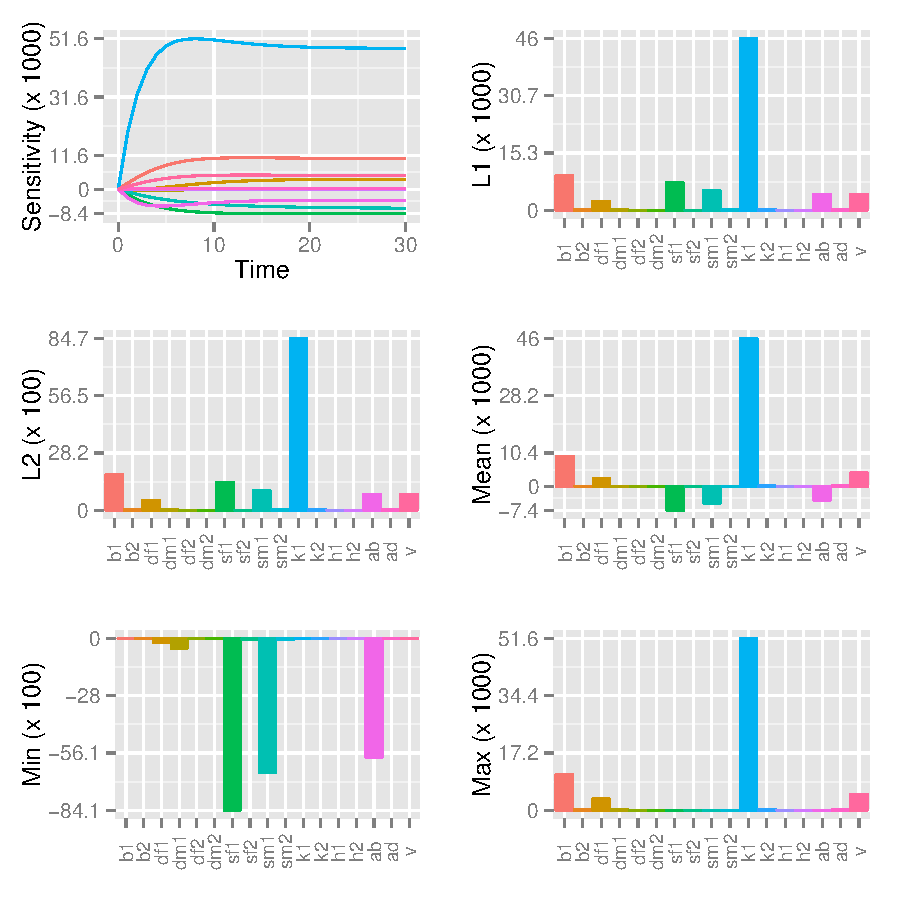
\includegraphics{capm_example-042}
\end{center}
\begin{Schunk}
\begin{Sinput}
> plotlocal(local.iasa.n2)
\end{Sinput}
\end{Schunk}
\begin{center}
\begin{Schunk}
\begin{Soutput}
%NULL
\end{Soutput}
\end{Schunk}
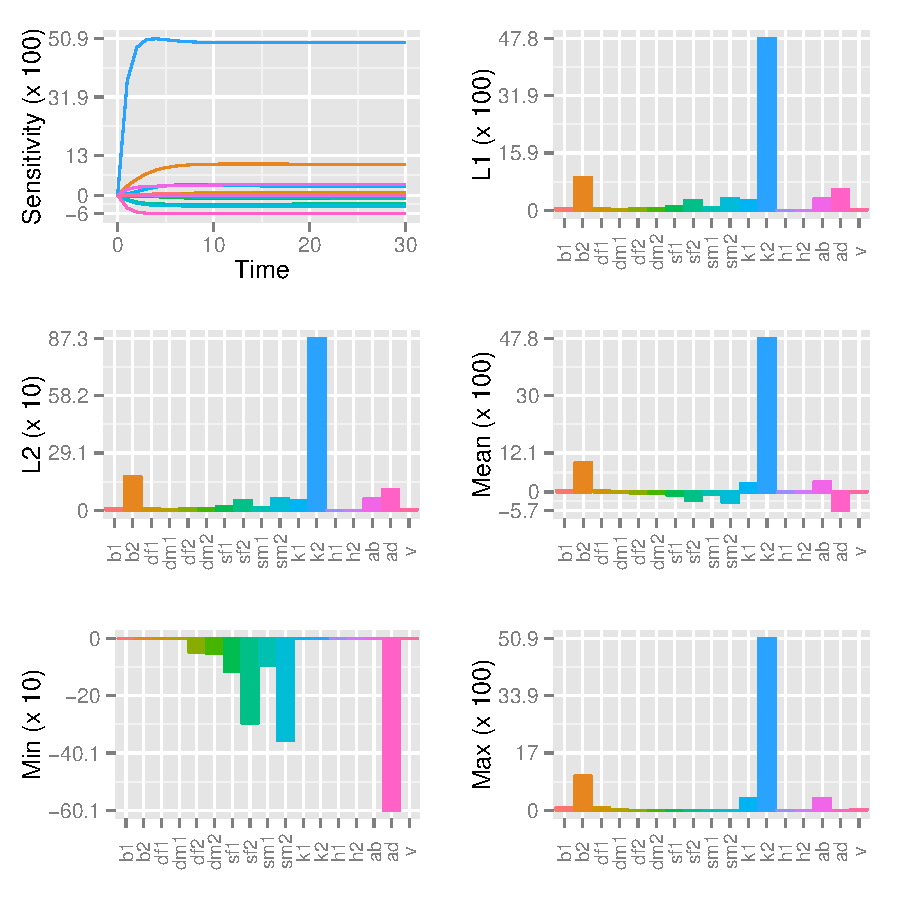
\includegraphics{capm_example-044}
\end{center}
\subsection{Create scenarios of intervention}
To end your first analysis, create intervention scenarios to assess the effect of different combinations of sterilization, abandonment, adoption and replacement rates. Define the minimum and maximum for each of this rates and run the model (can take few seconds or maybe minutes)

\begin{Schunk}
\begin{Sinput}
> iasa.rg <- iasa(pars = pars.iasa,
+                 state = state.iasa,
+                 time = 0:30,
+                 ster.range = seq(0, .5, length.out = 50),
+                 aban.range = c(0, .2),
+                 adop.range = c(0, .2),
+                 imm.range = c(0, .2))
\end{Sinput}
\end{Schunk}

and plot the results.
\subsection{Local sensitivity analysis}
As a complement for global sensitivity analysis, local sensitivities allow the ranking of parameters according to their importance. Instead of using ranges, local sensitivities assess the parameters in a small space around the point estimates using the so-called sensitivity functions.

\begin{Schunk}
\begin{Sinput}
> local.iasa.n1 = localsens(model.out = iasa.pt, sensv = 'N1')
> head(local.iasa.n1)
\end{Sinput}
\begin{Soutput}
  x var       b1        b2       df1        dm1        df2        dm2
1 0  N1    0.000  0.000000     0.000     0.0000  0.0000000  0.0000000
2 1  N1 2087.049  1.228182 -1259.434  -892.1073 -0.1603598 -0.1697615
3 2  N1 4171.552  3.729656 -2178.732 -1572.5255 -0.5026907 -0.5332427
4 3  N1 6069.342  7.334165 -2820.156 -2075.6284 -0.9198440 -0.9802356
5 4  N1 7701.632 11.695374 -3247.613 -2438.8060 -1.3371790 -1.4345872
6 5  N1 9052.026 16.351987 -3517.119 -2695.8193 -1.7120177 -1.8540281
         sf1        sf2        sm1        sm2       k1        k2 h1 h2
1    0.00000  0.0000000    0.00000  0.0000000     0.00   0.00000  0  0
2  -85.85013 -0.1001899  -38.40532 -0.1055014 20196.14  29.25517  0  0
3 -271.29587 -0.8085772 -124.96069 -0.8468487 34394.12  84.20611  0  0
4 -486.58474 -1.9974686 -230.81144 -2.1352753 44186.88 141.72256  0  0
5 -695.69408 -3.3742981 -339.92092 -3.6822894 50830.62 192.04890  0  0
6 -882.13908 -4.7144567 -443.98950 -5.2494579 55268.25 232.67057  0  0
         ab        ad         v
1     0.000   0.00000    0.0000
2 -3971.651  66.44725  935.6548
3 -6594.534 128.39664 1870.1688
4 -8279.184 182.33433 2720.9759
5 -9328.786 227.35097 3452.7556
6 -9958.749 263.78839 4058.1575
\end{Soutput}
\begin{Sinput}
> summary(local.iasa.n1)
\end{Sinput}
\begin{Soutput}
      value   scale      L1      L2     Mean      Min     Max  N
b1  2.2e+04 2.2e+04 1.1e+04 2.1e+03  1.1e+04      0.0 1.3e+04 31
b2  4.4e+03 4.4e+03 3.3e+01 6.4e+00  3.3e+01      0.0 4.3e+01 31
df1 1.0e-01 1.0e-01 3.2e+03 6.0e+02 -3.2e+03  -3779.8 0.0e+00 31
dm1 9.8e-02 9.8e-02 2.9e+03 5.4e+02 -2.9e+03  -3277.9 0.0e+00 31
df2 1.2e-01 1.2e-01 2.0e+00 3.8e-01 -2.0e+00     -2.7 0.0e+00 31
dm2 1.2e-01 1.2e-01 3.2e+00 6.2e-01 -3.2e+00     -4.5 0.0e+00 31
sf1 6.9e-02 6.9e-02 1.3e+03 2.5e+02 -1.3e+03  -1579.8 0.0e+00 31
sf2 5.0e-02 5.0e-02 7.2e+00 1.4e+00 -7.2e+00     -9.4 0.0e+00 31
sm1 2.8e-02 2.8e-02 8.5e+02 1.7e+02 -8.5e+02  -1186.3 0.0e+00 31
sm2 5.0e-02 5.0e-02 1.1e+01 2.3e+00 -1.1e+01    -16.8 0.0e+00 31
k1  9.8e+04 9.8e+04 5.7e+04 1.1e+04  5.7e+04      0.0 6.3e+04 31
k2  8.1e+03 8.1e+03 2.9e+02 5.5e+01  2.9e+02      0.0 3.4e+02 31
h1  1.0e+00 1.0e+00 1.4e-03 2.9e-04  1.4e-03      0.0 2.9e-03 31
h2  5.0e-01 5.0e-01 0.0e+00 0.0e+00  0.0e+00      0.0 0.0e+00 31
ab  5.4e-02 5.4e-02 9.7e+03 1.8e+03 -9.7e+03 -10615.4 0.0e+00 31
ad  1.0e-01 1.0e-01 3.2e+02 6.0e+01  3.2e+02      0.0 3.7e+02 31
v   1.0e-01 1.0e-01 5.1e+03 9.6e+02  5.1e+03      0.0 6.0e+03 31
\end{Soutput}
\begin{Sinput}
> local.iasa.n2 = localsens(model.out = iasa.pt, sensv = 'N2')
\end{Sinput}
\end{Schunk}

Ploting the results is straightforward as usual.
\begin{Schunk}
\begin{Sinput}
> plotlocal(local.iasa.n1)
\end{Sinput}
\end{Schunk}
\begin{center}
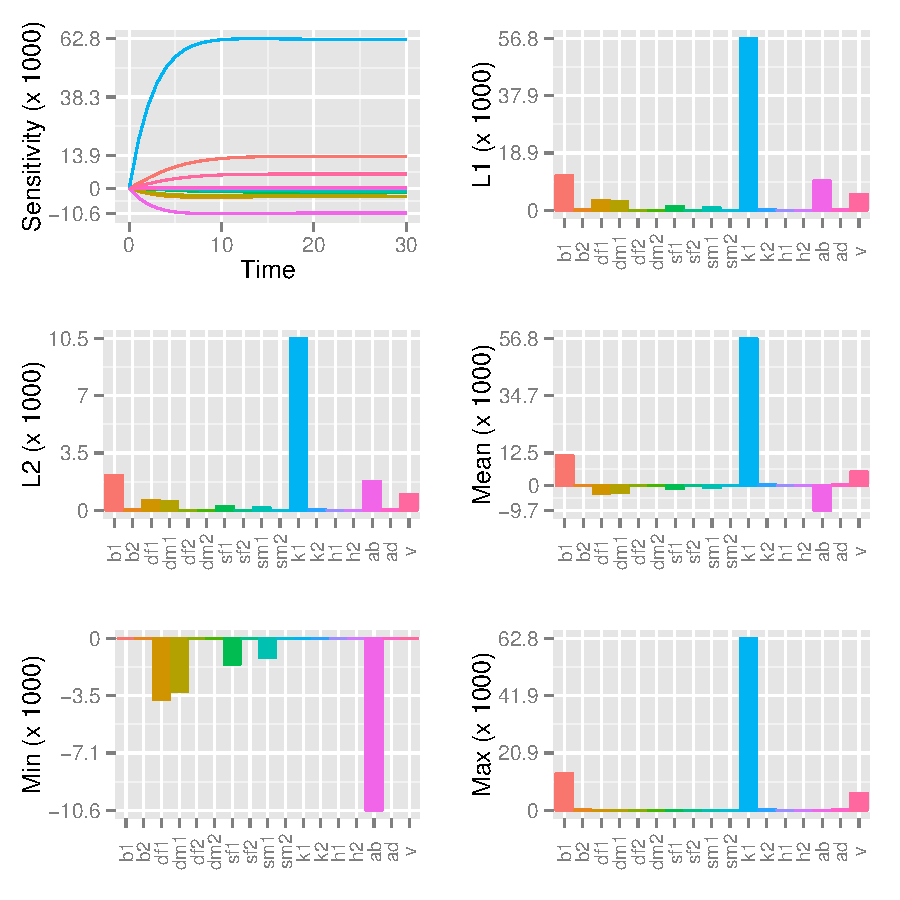
\includegraphics{capm_example-048}
\end{center}
\begin{Schunk}
\begin{Sinput}
> plotlocal(local.iasa.n2)
\end{Sinput}
\end{Schunk}
\begin{center}
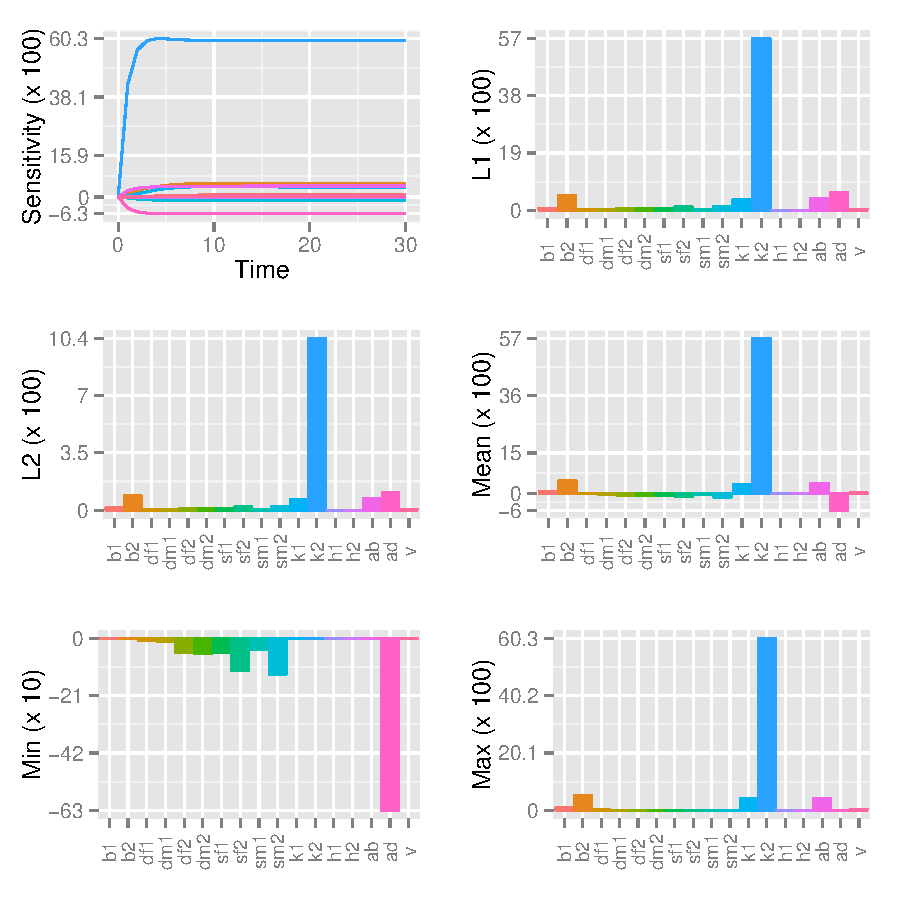
\includegraphics{capm_example-050}
\end{center}
\subsection{Create scenarios of intervention}
To end your first analysis, create intervention scenarios to assess the effect of different combinations of sterilization, abandonment, adoption and replacement rates. Define the minimum and maximum for each of this rates and run the model (can take few seconds or maybe minutes)

\begin{Schunk}
\begin{Sinput}
> iasa.rg <- iasa(pars = pars.iasa,
+                 state = state.iasa,
+                 time = 0:30,
+                 ster.range = seq(0, .5, length.out = 50),
+                 aban.range = c(0, .2),
+                 adop.range = c(0, .2),
+                 imm.range = c(0, .2))
\end{Sinput}
\end{Schunk}

and plot the results.

plotmodel(iasa.rg, variable = 'N')

\begin{center}
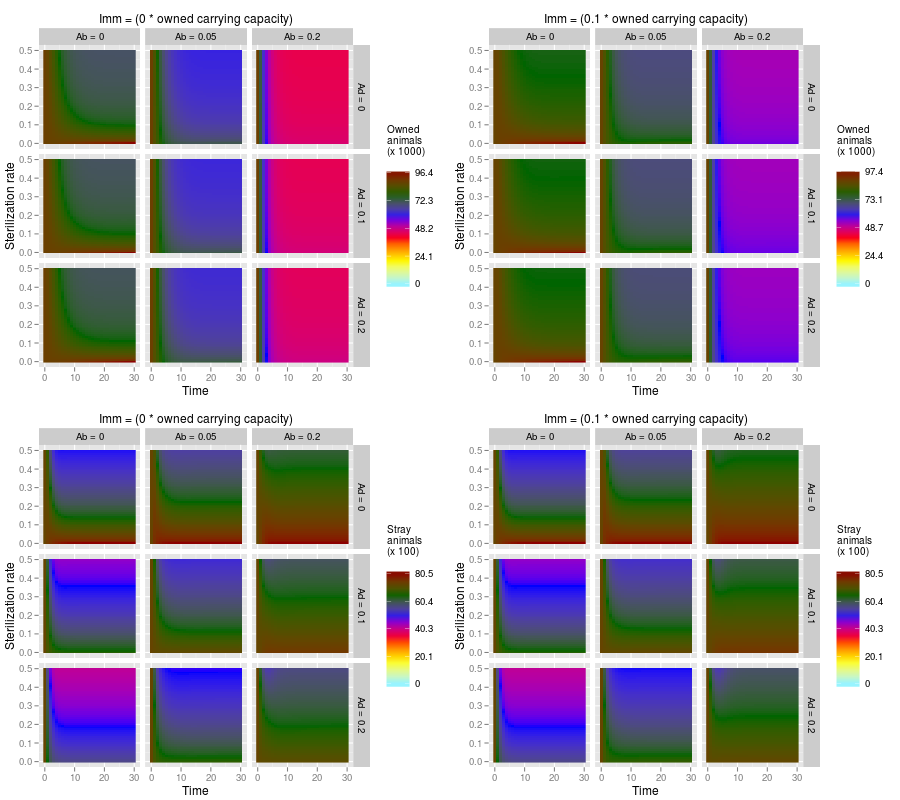
\includegraphics[scale=.9]{iasa_plot.png}
\end{center}


Abandonment rate produced noticeble changes in the size of both populations. Immigration rate reduced the effect of sterilization in owned population but did not prduced relevant changes in stray population. Sterilization and abandonment lost their impact on stray population size when there was abandonment.

plotmodel(iasa.rg, variable = 'n')

\begin{center}
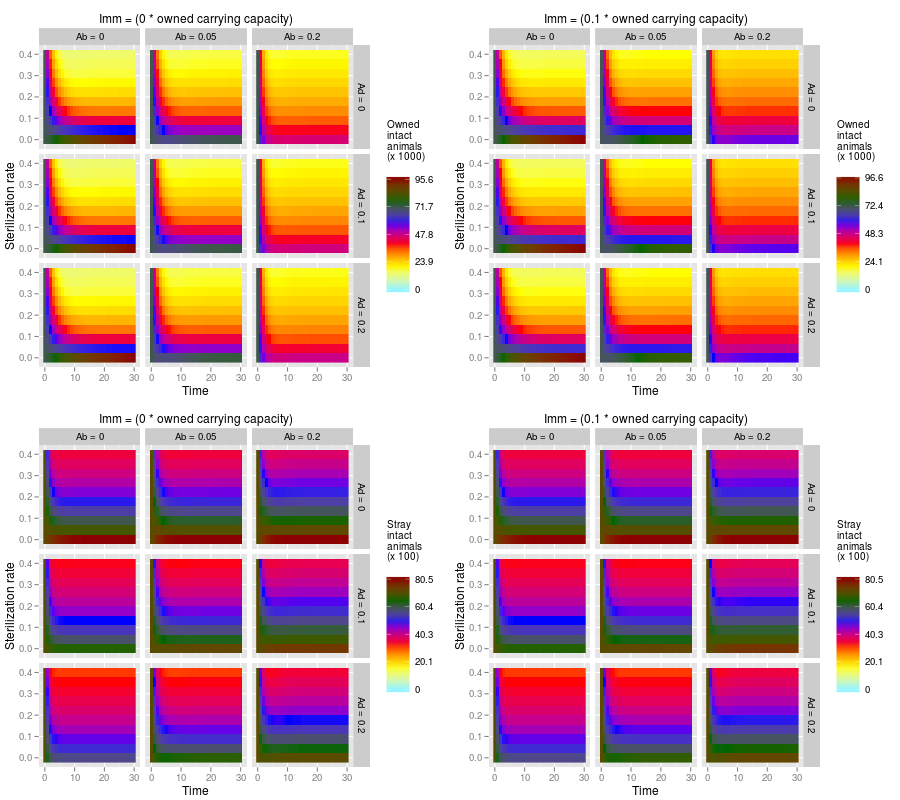
\includegraphics[scale=.9]{iasa_n.png}
\end{center}

plotmodel(iasa.rg, variable = 'cn')

\begin{center}
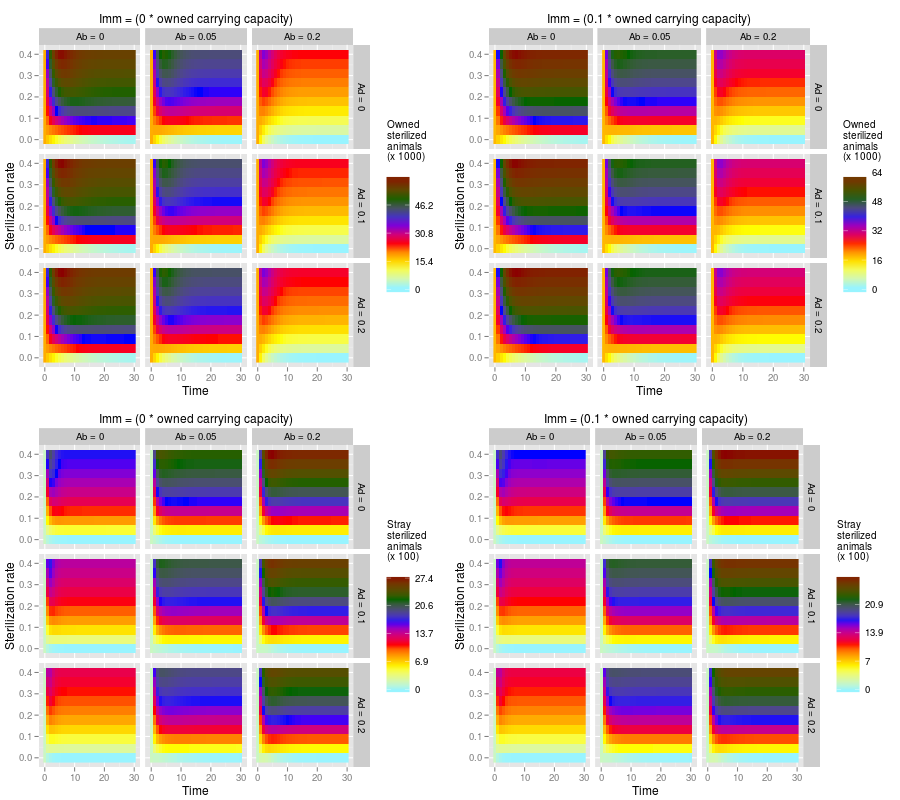
\includegraphics[scale=.9]{iasa_cn.png}
\end{center}


\end{document}
